\subsection{Tangent Measures of Pushforward Measures} \label{sec:pushforward}
Let $\mu \in \scrM(\bbR^m)$, and let $f \colon \bbR^m \to \bbR^d$ be a $C^1$ diffeomorphism. We would like to investigate the tangent measures of the pushforward measure $f_*\mu$. This investigation will follow many of the same lines as in section \ref{sec:submanifolds} Choose a tangent measure $\tau \in \Tan(\mu,q)$, and let $c_j \mu_{q,r_j}$ be a blowup sequence for $\tau$. By translating if necessary, we may assume $f(q) = 0$. Fix $\phi \in C_c(\bbR^d)$, and let $R > 0$ be such that $\supp{\phi} \subseteq B(0,R)$. Consider now 
\begin{equation} \begin{aligned}
    c_j \int_{\bbR^d} \phi \; \d(f_*\mu)_{0,r_j} &= c_j \int_{\bbR^d} \phi\parens{\frac{x}{r_j}} \; \d(f_* \mu)(x) \\
                                               &= c_j \int_{\bbR^m} \phi\parens{\frac{f(y)}{r_j}} \; \d\mu(y).
\end{aligned} \end{equation}
Note that since $f$ is a diffeomorphism, the set $f^{-1}(B(0,R))$ is bounded, so $f$ is uniformly Lipschitz on this set. Let $\Lip{f}$ be its Lipschitz constant on this set. If $y \in \bbR^m$ lies outside the set $B(0,rR/\Lip{f})$, then $f(y)/r$ lies outside the set $B(0,R)$ (again, cf. section \ref{sec:submanifolds}). So for $K := R/\Lip{f}$, the above integral is 
\begin{equation}
    c_j \int_{B(0,Kr_j)} \phi\parens{\frac{f(y)}{r_j}} \; \d\mu{y}.
\end{equation}
Now, we also have 
\begin{equation} \begin{aligned}
    &\lim_{j \to \infty} \abs{ c_j \int_{B(0,Kr_j)} \phi\parens{\frac{f(y)}{r_j}} \; \d\mu(y) - c_j \int_{B(0,Kr_j)} \phi\parens{\frac{\d f(0)(y)}{r_j}} \; \d\mu(y) } \\
    &\quad \leq \lim_{j \to \infty} c_j \mu(0,Kr_j) \, C \sup_{y \in B(0,Kr_j)} \frac{\abs{f(y) - \d f(0)(y)}}{r_j} \\
    &= 0,
\end{aligned} \end{equation}
where $C > 0$ is the Lipschitz constant of $\phi$. Here, we remark that by our study of the normalizing constants $c_j$ in section \ref{sec:blowingUp}, we may take $c_j = \mu(B(0,Kr_j))^{-1}$ without loss of generality, and the resulting tangent measure will be the same up to multiplication by a constant. This is of course inconsequential, since $\Tan(f_*\mu,0)$ is a cone by lemma \ref{lem:tangent_measure_properties}. Finally, we then have 
\begin{equation} \begin{aligned}
    \lim_{j \to \infty} c_j \int_{B(0,Kr_j)} \phi\parens{\frac{\d f(0)(y)}{r_j}} \; \d\mu(y) &= \lim_{j \to \infty} c_j \int_{\bbR^m} \phi\parens{\frac{\d f(0)(y)}{r_j}} \; \d\mu(y) \\
    &= \int_{\bbR^m} \phi\parens{ \d f(0)(y) } \; \d\tau(y) \\
    &= \int_{\bbR^d} \phi \; \d(\d f(0)_* \tau).
\end{aligned} \end{equation}
It follows that $\d f(0)_*\tau$ is a tangent measure to $f_*\mu$ at $0$.

\begin{figure} 
    \centering
    \begin{tikzpicture}
        %\draw[gray] (0,0) grid (15,6);

        \draw[blue] (1,3) -- (5,3);
        \draw[blue] (11.5,3) circle (1.5cm);
        \draw[->] (6,3) to[out=30,in=150] (9,3);
        \node (f) at (7.5,4) {$f$};
        \node (L) at (3,2) {$\scrL^1 \restrict [0,2\pi)$};
        \node (HS) at (11.5,1) {$\scrH^1 \restrict S^1$};
        \filldraw[red] (4,3) circle (0.05cm);
        \node (q) at (4,3.5) {$q$};
        \filldraw[red] (11.5-1.06,3+1.06) circle (0.05cm);
        \node (p) at (11.5-1.06+0.4,3+1.06-0.4) {$p$};
        \draw[red] (11.5-1.06-1.06,3+1.06-1.06) -- (11.5-1.06+1.06,3+1.06+1.06);
        \node[anchor=east] (HTpS) at (11,5) {$\scrH^1 \restrict T_pS^1 = \d f(q)_* \scrL^1$};
    \end{tikzpicture}
    \caption{Pushforward of Lebesgue measure}
    \label{fig:pushforwardLebesgue}
\end{figure}

Let's consider the example suggested by figure \ref{fig:pushforwardLebesgue}. Define the map $f \colon [0,2\pi) \subseteq \bbR \to \bbR^2$ by $f(s) := (\cos{s},\sin{s})$, whose image is a circle. Recall the area formula (\ref{eq:areaFormula}). Since the derivative of $f$ at $s$ is just the (column) vector $f'(s) = (-\sin{s},\cos{s})$, we may calculate its Jacobian determinant to be
\begin{equation}
    \mathrm{J}f(s) = \sqrt{f'(s)^\T f'(s)} = 1.
\end{equation}
Given $\phi \in C_c(\bbR^2)$, we use the area formula to calculate 
\begin{equation} \begin{aligned}
    \int_{\bbR^2} \phi \; \d(\scrH^1 \restrict S^1) &= \int_{S^1} \phi \; \scrH^1 \\
    &= \int_0^{2\pi} \phi(f(s)) \J f(s) \; \d\scrL^1(s) \\
    &= \int_0^{2\pi} \phi(f(s)) \; \d\scrL^1(s) \\
    &= \int_\bbR \phi \; \d(f_*(\scrL^1 \restrict [0,2\pi)).
\end{aligned} \end{equation}
It follows that $\scrH^1 \restrict S^1$ is the pushforward measure $f_*\scrL^1$. Now fix a point $p = f(q) \in S^1$. In section \ref{sec:submanifolds}, we calculated that a tangent measure of $\scrH^1 \restrict S^1$ at $p$ is $\scrH^1 \restrict T_p S^1$. Our above calculations for tangent measures of pushforward measure shows that $\d f(q)_* \scrL^1$ is a tangent measure to $f_* (\scrL^1 \restrict [0,2\pi))$ at $p$. However, we know that $\d f(q)$ is given by $f'(q) = (-\sin{q},\cos{q})$, so the image of $\d f(q)$ is precisely the tangent space $T_p S^1$. Using the area formula again, we see that our theory from this section and section \ref{sec:submanifolds} do not contradict each other.


\subsection{Hausdorff Density and Singularities}
Consider the measure $\mu = \delta_0 + \scrL^d$ on $\bbR^d$. Certainly, this measure is not singular with respect to $\scrL^d$ in the sense that its null sets are completely indistinct from those of Lebesgue measure, but there is certainly a problem at the origin. This invites us to consider defining a notion of ``singularity'' at a point in $\bbR^d$.

Recall the definition of Hausdorff density from section \ref{sec:rectifiability}. Immediately from the defition, we see $\Theta^d(\scrL^d,p) = \omega_d$ for all $p \in \bbR^d$, where $\omega_d$ is the volume of the unit ball in $\bbR^d$. Some authors put a constant in the denominator of the definition of the upper and lower Hausdorff densities to ensure $\Theta^d(\scrL^d,p) = 1$, but the exact value is not important, at least for our purposes. More generally, we have $\Theta^s(\scrH^s,p) = \omega_s$ for some $\omega_s > 0$. For our measure $\mu = \delta_0 + \scrL^d$ as above, it is easy to see that $\Theta^d(\mu,p) = \omega_d$ for $p \neq 0$, and $\Theta^d(\mu,0) = \infty$. 

Some simple properties of Hausdorff densities: {\color{red} do this}


Actually, David Preiss in {\bf [Preiss]} introduced tangent measures to prove the following long-standing conjecture {\color{red} was it long-standing?} in geometric measure theory:
\begin{theorem}[Marstrand]
    Let $\mu \in \scrM(\bbR^d)$ be a Radon measure. Suppose there exists $s > 0$ such that the Hausdorff density $\Theta^s(\mu,p)$ exists and is positive and finite for all $p$ in a set of positive $\mu$-measure. Then $s$ is an integer.
\end{theorem}
In fact, Preiss proved the following stronger theorem:
\begin{theorem}[Preiss] \label{thm:preissMarstrand}
    Let $\mu \in \scrM(\bbR^d)$ be a Radon measure, and $k \in \bbN$ a positive integer. If the Hausdorff density $\Theta^k(\mu,p)$ exists and is positive and finite for all $p$ in the support of $\mu$, then $\mu$ is $k$-rectifiable.
\end{theorem}
Theorem \ref{thm:rectifiableFlatMeasures} says that it suffices to show this condition on the Hausdorff density implies we have flat tangent measures at $\mu$-a.e. point. See {\bf [de Lellis]} for a more thorough outline of the proof, or {\bf [Mattila chapter 14]} for  a direct proof of Marstrand's theorem.


\subsection{The Preiss Measure}
Our interest is showing that a partial converse to theorem \ref{thm:preissMarstrand} for $d=1$ is not true: namely, we can find a measure $\mu$ which has flat tangent measures at $\mu$-a.e. point, but whose Hausdorff 1-density at $\mu$-a.e. point is infinite. Stated as a theorem:
\begin{theorem}[Preiss]
    There exists a Radon measure $\mu \in \scrM(\bbR)$ such that for $\mu$-a.e. $p \in \bbR$, we have $\Theta^{1*}(\mu,p) = \infty$, and $\Tan(\mu,p) = \set{c \scrL^1 : c > 0}$.
\end{theorem}
We will sketch a proof of this theorem here, details can be found in {\bf [Preiss 5.8]}.

As was the case with the O'Neil measure, the Preiss measure will be of the form $\mu = f_* \scrL \restrict (0,1)$ for some function $f \colon (0,1) \to \bbR$. To motivate the proof, let's determine what $f$ should look like. By our calculations in section \ref{sec:pushforward}, we would like any notion of gradient of $f$ to be somewhat constant. On the other hand, the singularity condition $\Theta^{1*}(\mu,p) = \infty$ means the Lebesgue measure of $f^{-1}(B(p,r))$ should be approximately $r^{1-\epsilon}$ for some small $\epsilon \in (0,1)$.

The construction employed is dyadic. We will construct a sequence of approximate gradients of $f$, and show their antiderivatives converge to the thing we're looking for. We will try to find $\mu$ directly satisfying the singularity condition 
\begin{equation}
    \Theta^{1\ast}(\mu,f(t)) = \limsup_{r \downarrow \infty} \frac{\mu(B(f(t),r))}{r} = \infty \quad \text{for } \scrL^1\text{-a.e. } t \in (0,1),
\end{equation}

and for $\scrL^1$-a.e. $t \in (0,1)$ and $\tau \in \Tan(\mu,f(t))$, we want to find $c > 0$ such that $\Theta^{1}(\tau,p) = c$ for all $p \in \bbR$. Indeed, this implies 
\begin{equation}
    \frac{\d\tau}{\d\scrL^1}(p) = c,
\end{equation}
for all $p \in \bbR$, so by the Besicovitch differentiation theorem (theorem \ref{thm:besicovitch}), we must have $\tau = c\scrL^1$.

Having discussed our motivation for the construction, let's begin the construction. This construction will be based on a collection of dyadic subintervals of $[0,1)$ of the form $[i2^{-k},(i+1)2^{-k})$. We will define them rigourously by induction. To start let $Q := [0,1)$. Next, given $Q_{i_1,\dots,i_{k-1}} \subseteq Q$ define $Q_{i_1,\dots,i_{k-1},0}$ to be the first half-open subinterval of $Q_{i_1,\dots,i_{k-1}}$ of size $2^{-k}$, and $Q_{i_1,\dots,i_{k-1},1}$ to be the second. The construction intervals $Q_i$ are therefore enumerated by binary sequences $i = (i_1,\dots,i_k) \in \set{0,1}^k$. The integer $k$ is called the \textit{generation} of the interval $Q_i$. The \textit{children} of $Q_i$ are $Q_{i0}$ and $Q_{i1}$, and $Q_i$ is the children's \textit{parent}. Given a binary sequence $i = (i_1,\dots,i_k)$, its \textit{parity} $\abs{i}$ is defined to be the sum $i_{k-1} + i_k$, with addition taken mod 2. For example, the parity of the sequence $011010$ is $1$, and the parity of $1010111$ is $1 + 1 = 0$. See figure \ref{fig:binaryIntervals}.

\begin{figure}
    \centering
    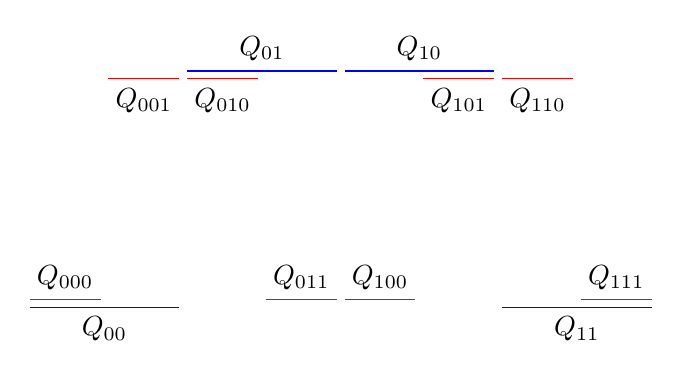
\begin{tikzpicture}
        %\draw[gray] (0,0) grid (10,5);

        \draw[blue] (0.05,0) -- (1.95,0) (2.05,3) -- (3.95,3) (4.05,3) -- (5.95,3) (6.05,0) -- (7.95,0);
        \draw[red] (0.05,0.1) -- (0.95,0.1) (1.05,2.9) -- (1.95,2.9) (2.05,2.9) -- (2.95,2.9) (3.05,0.1) -- (3.95,0.1) (4.05,0.1) -- (4.95,0.1) (5.05,2.9) -- (5.95,2.9) (6.05,2.9) -- (6.95,2.9) (7.05,0.1) -- (7.95,0.1);

        \draw node[above] at (0.5,0.1) {$Q_{000}$} node[below] at (1.5,2.9) {$Q_{001}$} node[below] at (2.5,2.9) {$Q_{010}$} node[above] at (3.5,0.1) {$Q_{011}$} node[above] at (4.5,0.1) {$Q_{100}$} node[below] at (5.5,2.9) {$Q_{101}$} node[below] at (6.5,2.9) {$Q_{110}$} node[above] at (7.5,0.1) {$Q_{111}$};

        \draw node[below] at (1,0) {$Q_{00}$} node[above] at (3,3) {$Q_{01}$} node[above] at (5,3) {$Q_{10}$} node[below] at (7,0) {$Q_{11}$};
    \end{tikzpicture}
    \caption{Construction intervals and corresponding parity}
    \label{fig:binaryIntervals}
\end{figure}

Having defined the construction intervals, we define the functions $g_k \colon Q \to \bbR$ inductively. In effect, $g_k$ is defined by a sequence of ``microadjustments''. Define $g_0 \colon Q \to \bbR$ by $g_0(t) = 1$ for all $t \in Q$, and fix $\epsilon_0 \in (0,1)$. Suppose $g_{k-1}$ and $\epsilon_{k-1}$ have been defined, and set 
\begin{equation}
    g_k(t) := \parens{1 + \sum_{i \in \set{0,1}^k} s_i \bbone_{Q_i}(t)} g_{k-1}(t),
\end{equation}
where $s_i = 0$ if $\abs{g_{k-1}(s)} < \epsilon_{k-1}$ for some (hence all) $s$ in the parent of $Q_i$, and $s_i = (-1)^{\abs{i}} \epsilon_{k-1}$ otherwise. We also let $\epsilon_k = \epsilon_{k-1}$ if 
\begin{equation} \begin{aligned}
    &\quad \abs{\set{t \in Q : \abs{g_{j-1}(t)} > \epsilon_{k-1} \text{ for } j = 0,\dots,k-1}} \geq \epsilon_{k-1} \\
    & \text{ or } \abs{\set{t \in Q : \abs{g_{k-1}(t)} \leq 1 \text{ for } j = 0,\dots,k-1}} \geq \epsilon_{k-1},
\end{aligned} \end{equation}
and $\epsilon_k = \epsilon_{k-1}/2$ otherwise. We also set 
\begin{equation}
    f_k(t) := \int_0^t g_k(s) \; \d s.
\end{equation}
See figure \ref{fig:iterationsOfG} for some iterations of $g$.

\begin{figure}
    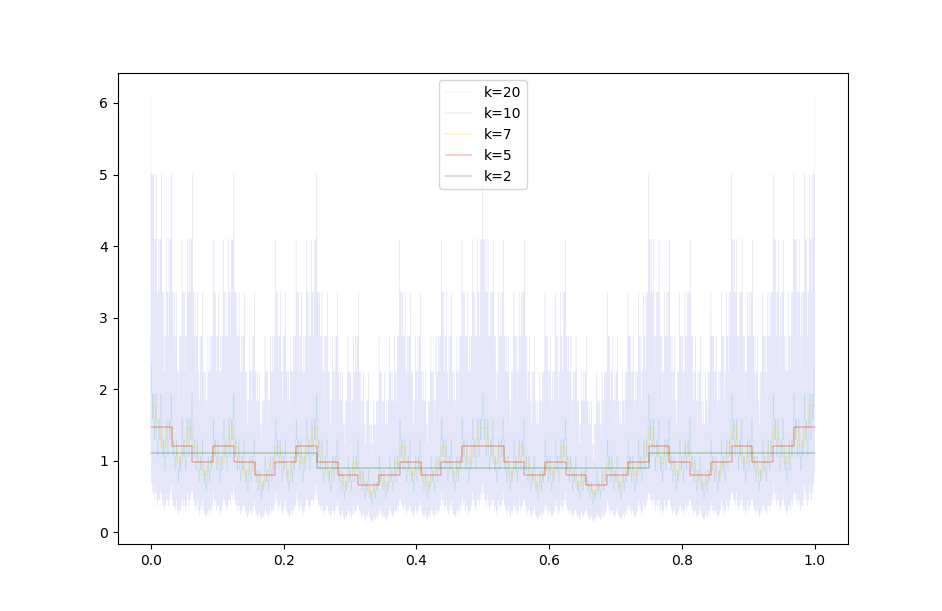
\includegraphics[width=\textwidth]{Figure_3.png}
    %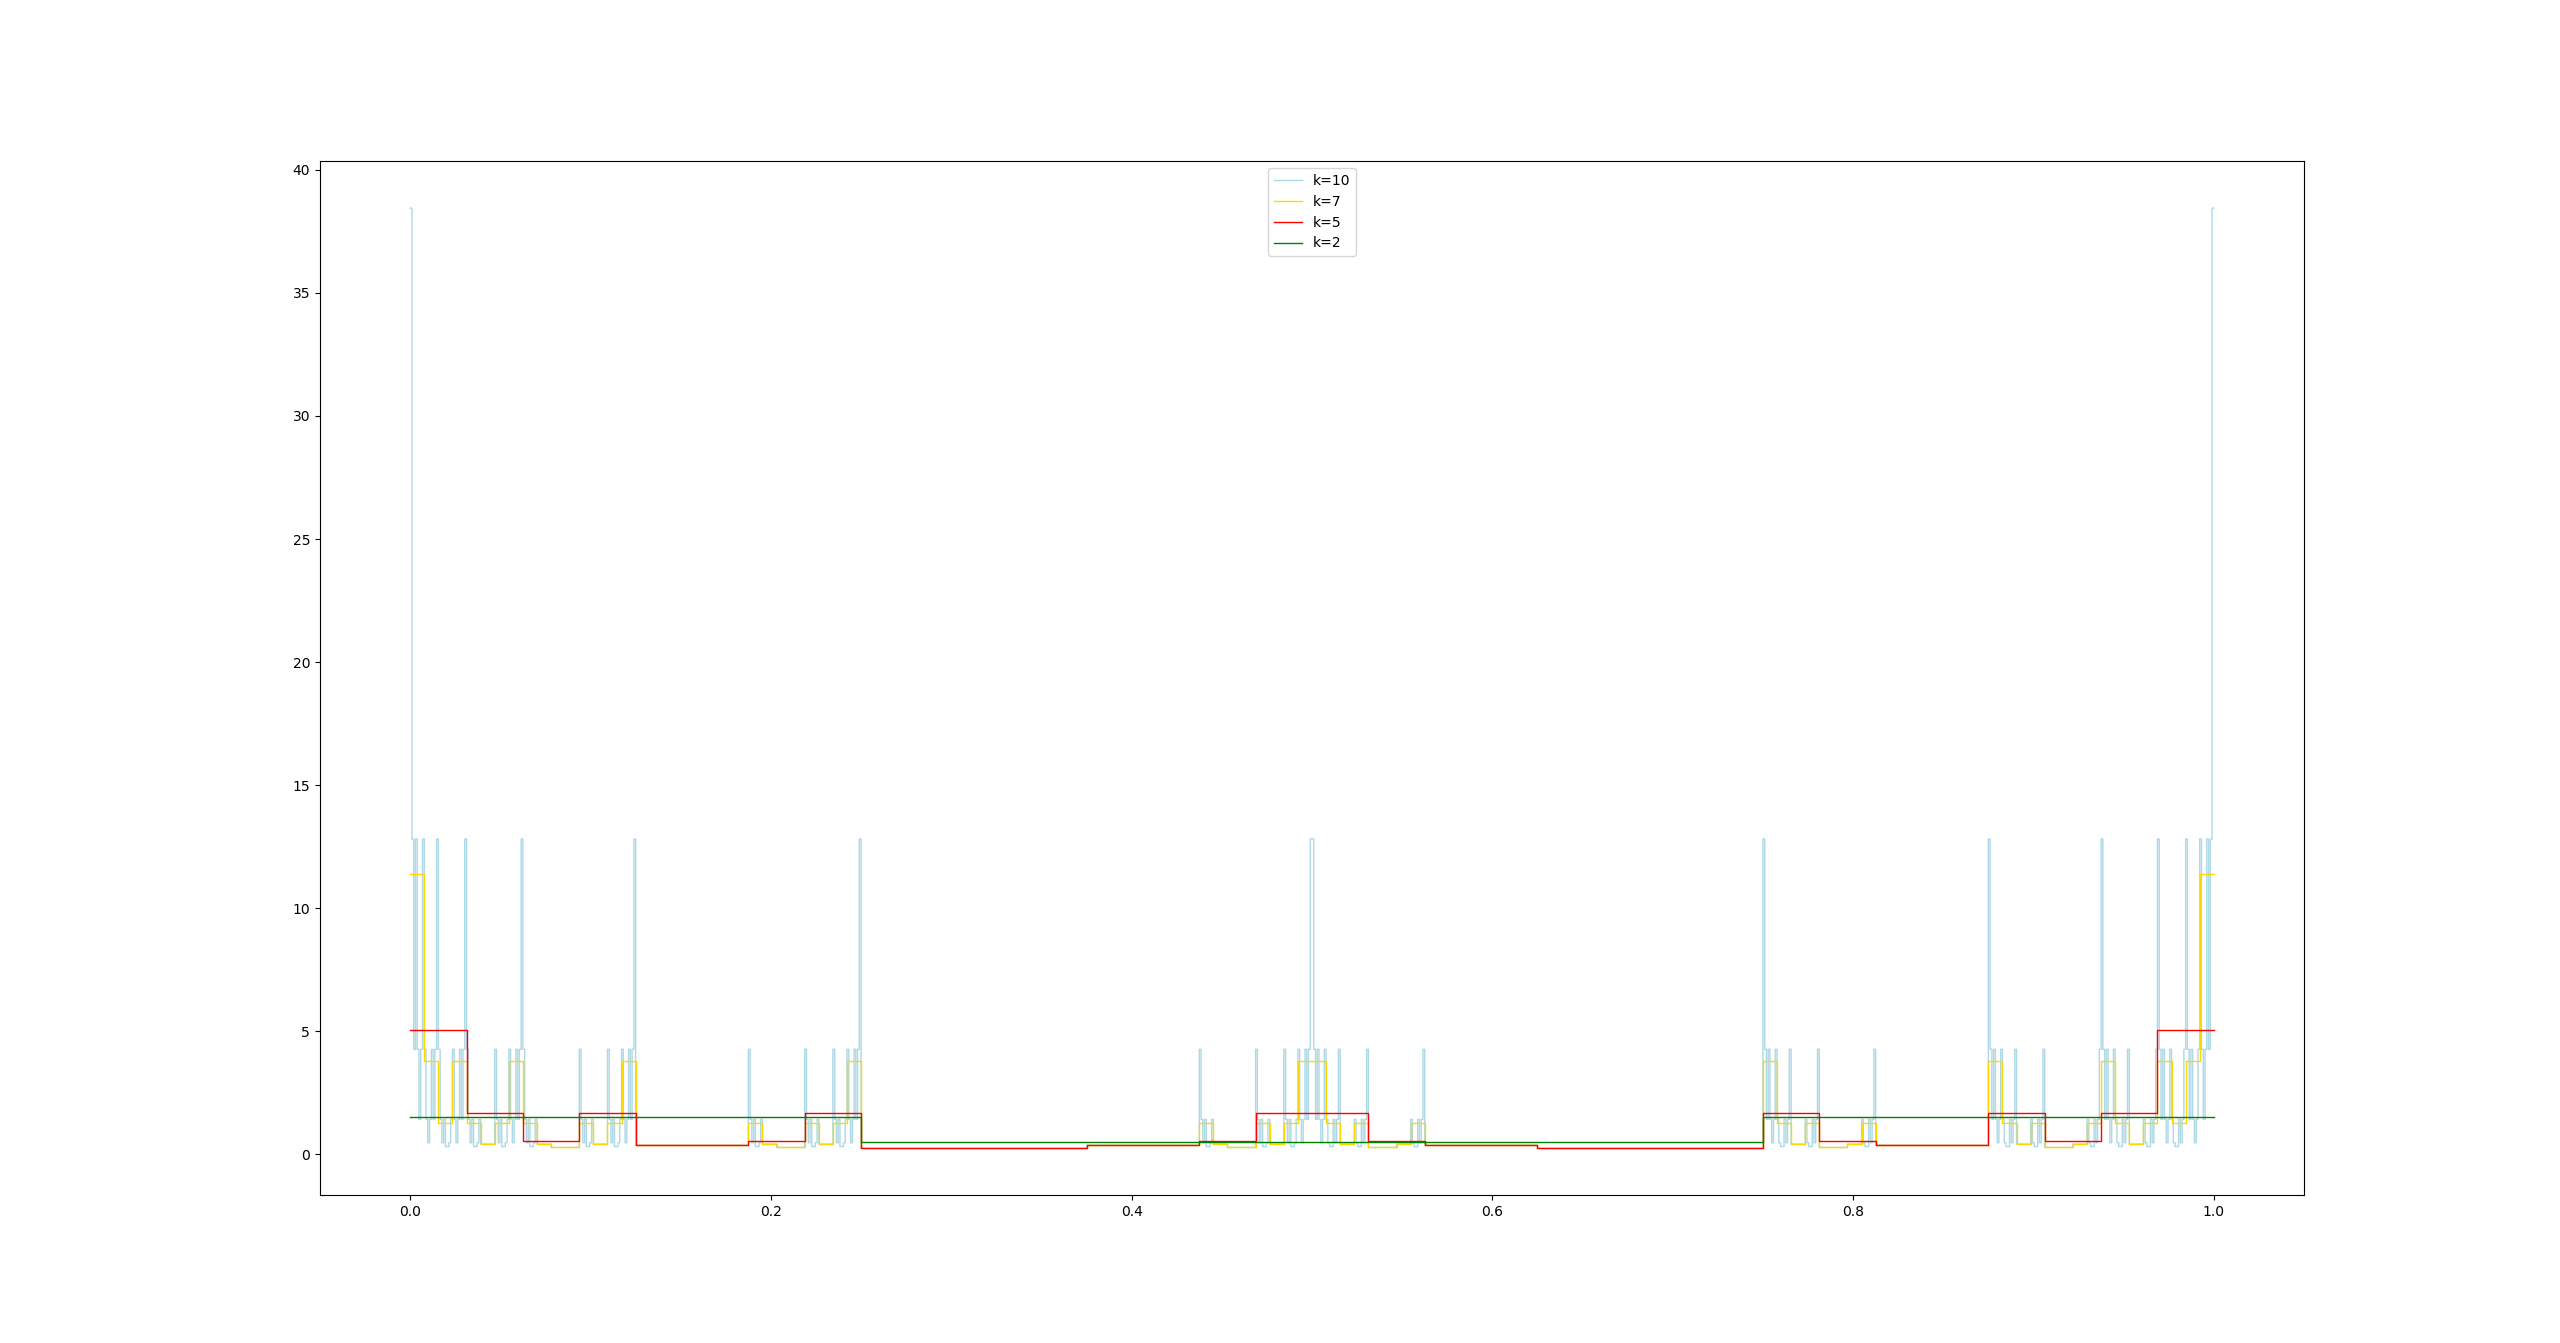
\includegraphics[width=0.5\textwidth]{iterationsOfGEpsilonLarge.png}
    
    \caption{Some iterations of $g_k$ for $\epsilon_0 = 0.1$.}
    \label{fig:iterationsOfG}
\end{figure}

Now, for all construction intervals $Q_i$ of generation $k$, we have $f_{k+1}(t) = f_k(t)$ whenever $s$ is one of the endpoints of $Q_i$ {\color{red} detailify this by using definition of $s_i$}. Fix $t \in Q$, and let $Q_i = [a,b)$ be the generation $k$ construction interval in which $t$ lies. Then 
\begin{equation} \begin{aligned}
    f_{k+1}(t) - f_k(t) &= \int_0^t g_{k+1}(s) - g_k(s) \; \d s \\
                        &= \int_a^t g_{k+1}(s) - g_k(s) \; \d s \\
                        &\leq \int_a^t \epsilon_k g_k(s) \; \d s \\
                        &= (t-a) \epsilon_k g_k(a) \\
                        &\leq 2^{-k} \epsilon_k (1 + \epsilon_0)^k,
\end{aligned} \end{equation}
since $g_k$ is constant on $[a,t)$. Taking suprema over $t \in [0,1]$, it follows that $\norm{f_{k+1} - f_k}_{L^\infty} \leq 2^{-k} \epsilon_0 (1 + \epsilon_0)^k$. Since $\sum_{k=1}^\infty \parens{\frac{1+\epsilon_0}{2}}^k < \infty$, the sequence $f_k$ is Cauchy in $C([0,1])$, so converges uniformly to some $f \in C([0,1])$. 

The aim now is to show $\mu := f_* \scrL^1 \restrict Q$ is the measure we want. This will follow by finding a function $h \colon Q \times (0,\infty) \to (0,\infty)$ such that for $\scrL^1$-a.e. $t \in Q$, we have
\begin{enumerate}[label=(\arabic*)] 
    \item \begin{equation} \label{eq:asymptoticEquiv}
        \lim_{r \downarrow 0} \frac{\mu(B(f(t),r))}{h(t,r)} = 1,
    \end{equation}

    \item \begin{equation} \label{eq:singular}
        \limsup_{r \downarrow 0} \frac{h(t,r)}{r} = \infty, \text{ and}
    \end{equation}

    \item \begin{equation} \label{eq:uniformity}
        \lim_{r \downarrow 0} \frac{h(t,sr)}{h(t,r)} = s \text{ for all } s > 0.
    \end{equation}
\end{enumerate}
Indeed, (1) and (2) immediately imply $\Theta^{1*}(\mu,f(t)) = \infty$. Meanwhile for $\tau \in \Tan(\mu,f(t))$ with $c\mu(B(f(t),r_j)^{-1} \mu_{f(t),r_j} \weakstar \tau$, we use lemma \ref{lem:semicontinuityOfWeak*Convergence}, (1), and (3) to calculate
\begin{equation} \begin{aligned}
    \Theta^1(\tau,0) &= \lim_{r \downarrow 0} \frac{\tau(B(0,r))}{r} \\
                     &\leq \lim_{r \downarrow 0} \liminf_{j \to \infty} \frac{c \mu_{f(t),r_j}(B(0,r))}{r\mu(B(f(t),r_j))} \\
                     &= \lim_{r \downarrow 0} \liminf_{j \to \infty} \frac{c}{r} \frac{ h(t,r_j) }{ \mu(B(f(t),r_j)) } \frac{ \mu(B(f(t),r_j r)) }{ h(t,r_j r) } \frac{ h(t,r_jr) }{ h(t,r_j) } \\
                     &= \lim_{r \downarrow 0} \frac{c}{r} r \\
                     &= c.
\end{aligned} \end{equation}
A similar calculation for $\tau(\overline{B(0,r)})$ is possible, which then shows $\Theta^1(\tau,0) = c$. To show $\Theta^1(\tau,p) = c$ for all other $p \in \bbR$, we {\color{red} do what? use continuity of $\mu$?}.

Let's now show such a function $h$ does exist. Immediately from the construction, we see
\begin{equation} \begin{aligned}
    g_k(t) &= \abs{1 + \sum_{i \in \set{0,1}^k} s_i \bbone_{Q_i}(t)} \abs{g_{k-1}(t)} \\
                 &\leq (1 + \epsilon_k) \abs{1 + \sum_{i \in \set{0,1}^{k-1}} s_i \bbone_{Q_i}(t)} \abs{g_{k-2}(t)} \\
                 &\leq \cdots \\
                 &\leq \prod_{j=1}^k (1 + \epsilon_k) \\
                 &\leq (1 + \epsilon_0)^k
\end{aligned} \end{equation}
for all $t \in Q$ and $k \in \bbN$, and $g_k(t) \geq (1 - \epsilon_0)^k$ similarly.

We would like to find a subsequence $g_{k_j}$ along which $\epsilon_{k_j+1} = \epsilon_{k_j}/2$. Suppose, for a contradiction, that there does not exist such a subsequence. Then the sequence $\epsilon_k$ eventually stabilizes, so we can choose $k_0 \in \bbN$ such that $\epsilon_k = \epsilon_{k_0}$ for all $k \geq k_0$. Then either $\abs{ \set{t \in Q : \abs{g_k(t)} > \epsilon_{k_0} \text{ for all } k }} > 0$, or $\abs{ \set{t \in Q : \abs{g_k(t)} \leq 1 \text{ for all } k }} > 0$. Indeed, this is since 
\begin{equation}
    \abs{ \set{ t \in Q : \abs{g_k(t)} > \epsilon_{k_0} \text{ for all } k } } = \lim_{k \to \infty} \abs{ \set{ t \in Q : \abs{g_j(t)} > \epsilon_{k_0} \text{ for } j = 1,\dots,k } }
\end{equation}
and similarly for the other set. {\color{red} finish}

Having found $g_{k_j}$, by definition we see
\begin{equation}
    \abs{ \set{t \in Q : \abs{g_{k_j}(t)} > \epsilon_{k_j}} } < \epsilon_{k_j}
\end{equation}
for all $j \in \bbN$. Fix $\delta > 0$. Noting that $\lim_{j \to \infty} \epsilon_{k_j} = 0$, we have that for $j$ large enough,
\begin{equation}
    \abs{ \set{t \in Q : \abs{g_{k_j}(t)} > \delta } } \leq \abs{ \set{t \in Q : \abs{g_{k_j}(t)} > \epsilon_{k_j}} } \leq \epsilon_{k_j}.
\end{equation}
Letting $j \to \infty$ on both sides and recalling $\delta > 0$ was arbitrary, we conclude $g_{k_j} \to 0$ in measure. In particular, there exists a further subsequence (not relabeled) with $g_k \to 0$ a.e. Let $\widetilde{Q} \subseteq Q$ be the set of all $t$ with $g_k(t) \to 0$. From here on out, we will pass to this subsequence.

Given $t \in \widetilde{Q}$ and $r > 0$, define $k(t,r)$ to be the largest integer such that $\abs{g_k(t)} \geq 2^k r$. Note that $\lim_{r \downarrow 0} k(t,r) = \infty$ since, for all $K \in \bbN$, we can find $r > 0$ such that $2^{-K}(1+\epsilon_0)^K < r$. Define 
\begin{equation}
    h(t,r) := \frac{r}{g_{k(t,r)}(t)}
\end{equation}
Immediately, we see 
\begin{equation}
    \limsup_{r \downarrow 0} \frac{h(t,r)}{r} = \limsup_{r \downarrow 0} \frac{1}{g_{k(t,r)}(t)} = \infty,
\end{equation}
therefore proving (\ref{eq:singular}).

We next prove (\ref{eq:uniformity}). By definition of $h$, it suffices to show 
\begin{equation} \label{eq:uniformg}
    \lim_{r \downarrow 0} \frac{g_{k(t,r)}(t)}{g_{k(t,sr)}(t)} = 1 \text{ for all } s > 0.
\end{equation}
Suppose $s \in [\frac{1+\epsilon_0}{2},1]$. Then $k(t,r) \leq k(t,sr)$. Furthermore, if $j \geq k(t,r) + 2$, then 
\begin{equation} \begin{aligned}
    g_j(t) &\leq (1+\epsilon_0)^{j-k(t,r)-1}g_{k(t,r)+1}(t) \\
           &< (1 + \epsilon_0)^{j-k(t,r)-1}2^{k(t,r)+1}r \\
           &\leq \parens{\frac{1+\epsilon_0}{2}}^{j-k(t,r)-1} 2^j r \\
           &\leq 2^j sr. 
\end{aligned} \end{equation}
This implies $k(t,sr) \leq k(t,r) + 1$. Thanks to this, if $s \in [\frac{1+\epsilon_0}{2},1]$, then we have 
\begin{equation}
    (1-\epsilon_{k(t,r)+1}) g_{k(t,r)}(t) \leq g_{k(t,sr)}(t) \leq (1+\epsilon_{k(t,r)+1}) g_{k(t,r)}(t).
\end{equation}
Dividing through by $g_{k(t,r)}(t)$ and taking $r \downarrow 0$, noting $\epsilon_{k(t,r)} \to 0$, we conclude (\ref{eq:uniformg}) for $s \in [\frac{1+\epsilon_0}{2},1]$.

For all $k \in \bbN$ $s,t,v \in Q$ with $s < v < t$, we have 
\begin{equation}
    \abs{f_k(s) - f_k(t) - (s-t)g_k(v)} \leq \epsilon_{j-1} \abs{g_k(v)}(s-t),
\end{equation}
where $j \in \bbN$ is the smallest integer with $(s,t)$ not contained in some construction interval of generation $j$.





\subsection{Extensions and Concluding Remarks}
The Preiss measure was constructed to be a measure on $\bbR$. Indeed, the application of the integral on $[0,t]$ prevents our proof from extending to $\bbR^d$ for general $d$. One might then wonder if there exists an analog of the Preiss measure on $\bbR^d$ for $d \geq 2$. In fact, this is an open problem:
\begin{question}
    Let $d \geq 2$ be a positive integer. Does there exist $\mu \in \scrM(\bbR^d)$ such that $\Tan(\mu,x_0) = \set{c\scrL^d : c > 0}$ for $\mu$-a.e. $x_0 \in \bbR^d$?
\end{question}
While we will not be able to answer this here, we can provide some explanation for how a proof could be approached. Our construction of the Preiss measure on $\bbR$ relied fundamentally on lemma \ref{lem:asymptoticUniformityImpliesUniformityOfTangentMeasures} to show all tangent measures were $1$-uniform, and of course, the only $1$-uniform measures on $\bbR$ are $c\scrL^1$. The same is true more generally for $d$-uniform measures on $\bbR^d$. Indeed, suppose $\tau \in \scrM(\bbR^d)$ is $d$-uniform. {\color{red} show $\tau = c\scrL^d$.} It follows that if we can find a measure which is singular and asymptotically $d$-uniform, then we will have obtained our generalization of Preiss measure.

More generally, we could ask for a measure on $\bbR^d$ which is asymptotically $m$-uniform for some $m \neq d$. If $m > d$, then {\color{red} include a discussion on uniform measures including \texttt{https://arxiv.org/pdf/1608.02604.pdf, http://cvgmt.sns.it/media/doc/paper/4099/UniformMeasures.pdf, https://www.mscand.dk/article/view/14367}}

Recall the type of singularity we have constructed. That is, $\Theta^{1*}(\mu,x_0) = \infty$ for $\mu$-a.e. $x_0 \in \bbR$.

